\documentclass{article}
\usepackage{graphicx}
\graphicspath{ {images/} }

\title{Dynamic sampling pointnet notes}
\author{xyz}
\date{Feb 2018}

\begin{document}
%\tableofcontents{}
\begin{titlepage}
\maketitle
\end{titlepage}	

\section{Quick notes for important events while using one file to test}
\subsection{batch size}
\subsubsection{bs=27 vs bs=81}
batch size: 9,27,81 \par
data: xyz-color\_1norm\par
model: 1AG\par
sampling \& grouping: stride\_0d1\_step\_0d1\_bmap\_nh5\_2048\_0d5\_1\_fmn1-160\_32-32\_12-0d2\_0d6-0d2\_0d6\par
\begin{figure}[h]
	\caption{bs=9}
	\centering
	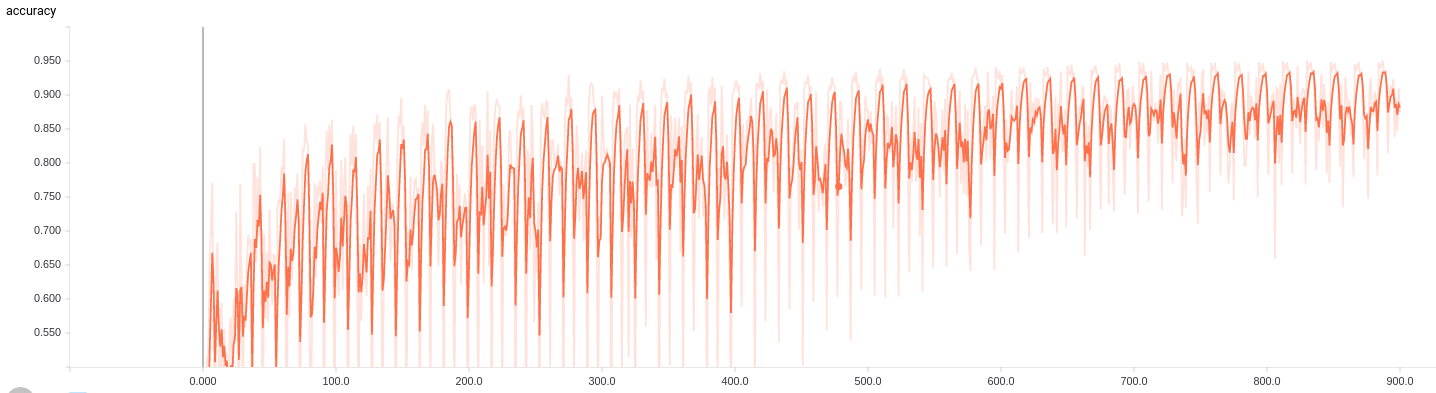
\includegraphics[width=\textwidth]{acc_log-model_1AG-gsbb_2C1-bs9-xyz-color_1norm-2048-mat}
	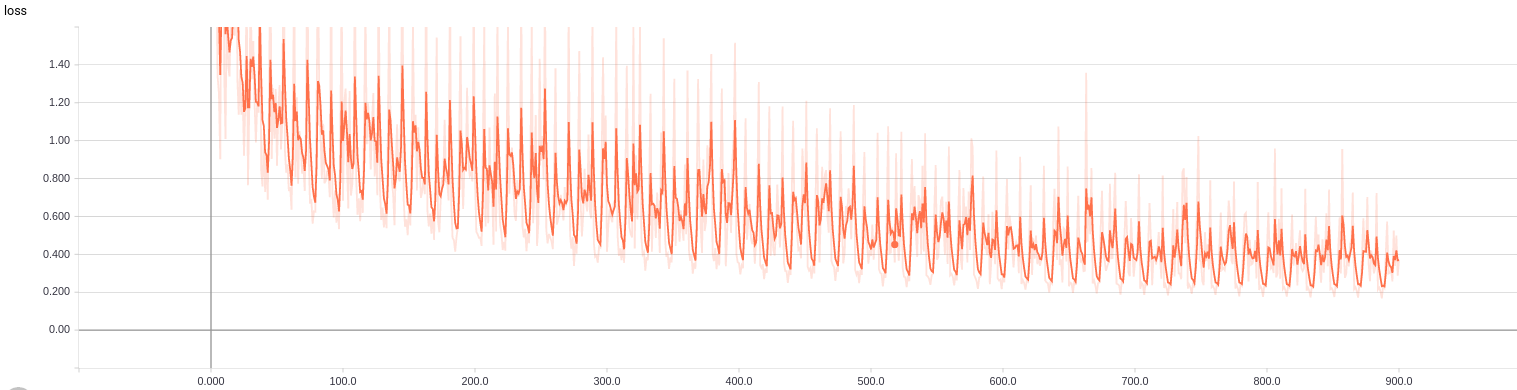
\includegraphics[width=\textwidth]{loss_log-model_1AG-gsbb_2C1-bs9-xyz-color_1norm-2048-mat}
\end{figure}
\begin{figure}[h]
	\caption{bs=27}
	\centering
	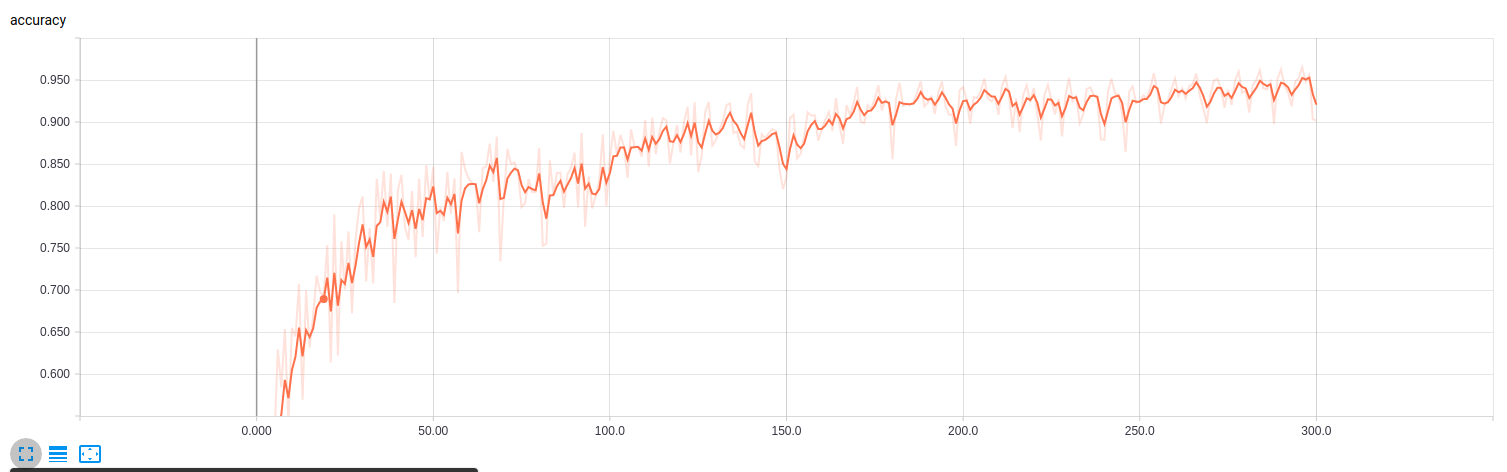
\includegraphics[width=\textwidth]{acc_log-model_1AG-gsbb_2C1-bs27-xyz-color_1norm-2048-mat}
	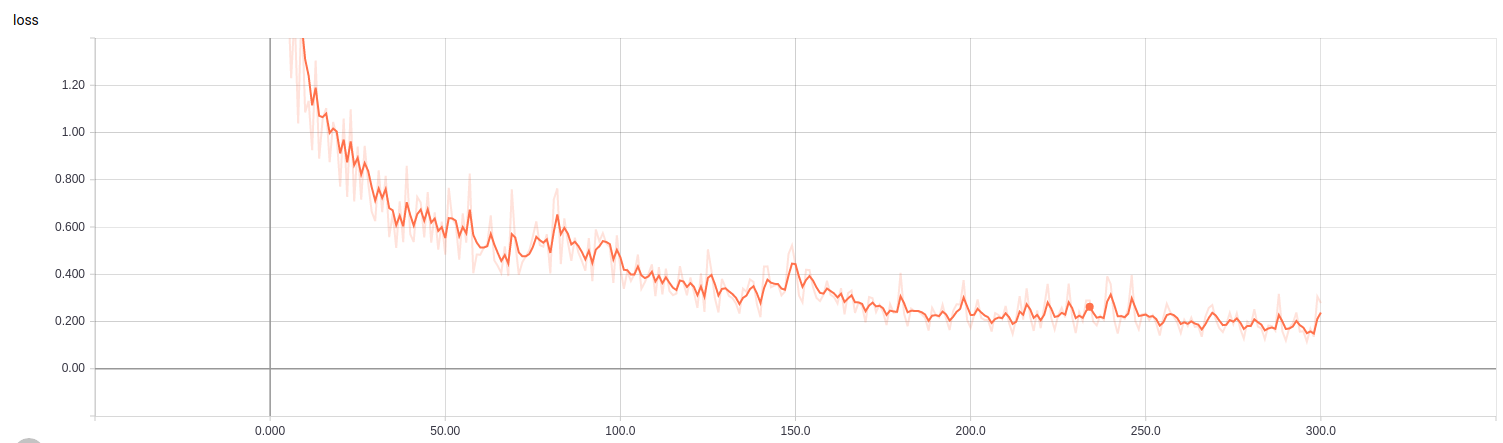
\includegraphics[width=\textwidth]{loss_log-model_1AG-gsbb_2C1-bs27-xyz-color_1norm-2048-mat}
\end{figure}
\begin{figure}[h]
	\centering
	\caption{bs=81}
	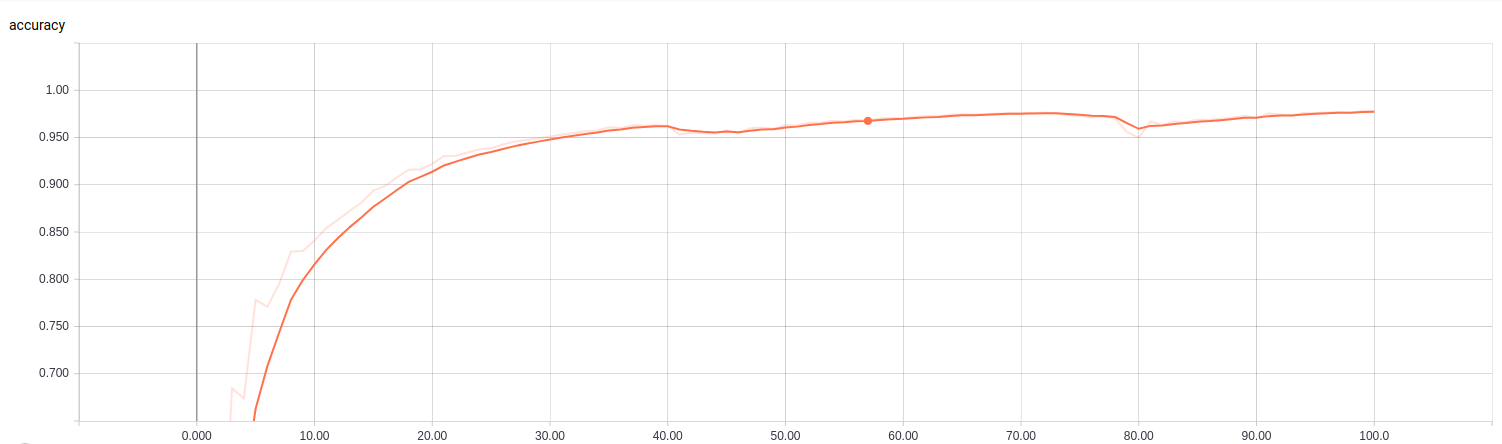
\includegraphics[width=\textwidth]{acc_log-model_1AG-gsbb_2C1-bs81-xyz-color_1norm-2048-mat}
	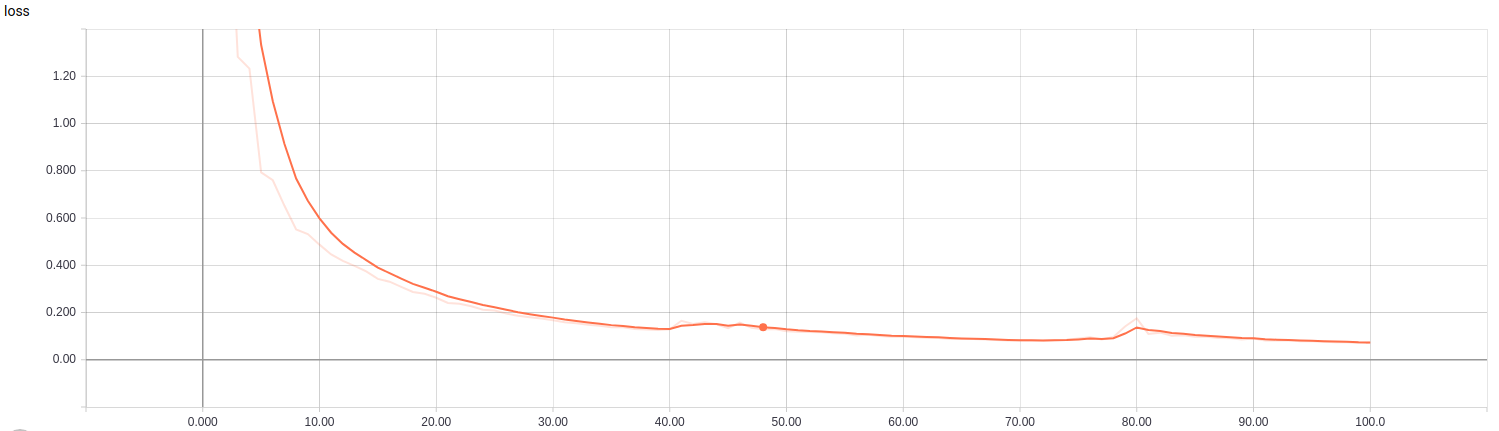
\includegraphics[width=\textwidth]{loss_log-model_1AG-gsbb_2C1-bs81-xyz-color_1norm-2048-mat}
\end{figure}
\subsection{feed elements}
epoch num = 100 \par
stride\_0d1\_step\_0d1\_bmap\_nh5\_2048\_0d5\_1\_fmn1-160\_32-32\_12-0d2\_0d6-0d2\_0d6 \par
\begin{center}
	\begin{tabular}{|c |c | c || c c |} 
		\hline
		model & batch size & data elements & acc & loss \\
		\hline
		1AG & 9 & xyz color & 0.890 & 0.356\\ [0.5ex] 
		\hline
		1AG & 27 & xyz color & 0.920 & 0.240\\ [0.5ex] 
		\hline
		
		3AG & 27 & xyz color& 0.912 & 0.273 \\  [0.5ex]
		\hline
		2A & 27 & xyz color& 0.908 & 0.294 \\  [0.5ex]
		\hline
		2AG & 27 & xyz color& 0.902 & 0.293 \\  [0.5ex]
		\hline
		1A & 27 & xyz color& 0.883 & 0.351 \\  [0.5ex]
		\hline
		1AG & 81 & xyz color & 0.978 & 0.072\\ [0.5ex] 
		\hline\hline
		
		1AG & 9 & xyz  & 0.861 & 0.427\\ [0.5ex] 
		\hline
		1AG & 27 & xyz & 0.907 & 0.257\\ [0.5ex] 
		\hline
		1AG & 81 & xyz & 0.975 & 0.078 \\  [0.5ex]
		\hline\hline
		1A & 27 & xyzmid color& 0.889 & 0.357 \\  [0.5ex]
		\hline
		3AG & 27 & xyzmid color& 0.933 & 0.193 \\  [0.5ex]
		\hline
		
		2A & 27 & xyzmid color& 0.939 & 0.177 \\  [0.5ex]
		\hline
		
		2AG & 27 & xyzmid color& 0.929 & 0.208 \\  [0.5ex]
		\hline\hline
		3AG & 27 & xyz xyzmid color& 0.924 & 0.230 \\  [0.5ex]
		\hline
		
		2A & 27 & xyz xyzmid color& 0.898 & 0.317 \\  [0.5ex]
		\hline
		2AG & 27 & xyz xyzmid color& 0.908 & 0.280 \\  [0.5ex]
		\hline
		1A & 27 & xyz xyzmid color& 0.910 & 0.281 \\  [0.5ex]
		\hline
		1AG & 27 & xyz xyzmid color& 0.944 & 0.163 \\  [0.5ex]
		\hline
		1AG & 81 & xyz xyzmid color& 0.976 & 0.078 \\  [0.5ex]
		\hline
		2A & 81 & xyz xyzmid color& 0.942 & 0.173 \\  [0.5ex]
		\hline
		3AG & 81 & xyz xyzmid color& 0.949 & 0.147 \\  [0.5ex]
		\hline
	\end{tabular}
\end{center}

1. large batch size is better \par
2. $1AG (0.92) > 3AG(0.912) > 2A(0.908) > 2AG(0.902) > 1A(883)$ \par
   1AG is much better than 1A \par 
   \textbf{1AG is a bit better than 3AG ???} \par

3. xyz-color is only a bit better than xyz \par
4. xyzmid-color is much better than xyz-color \par
5. \textbf{xyzmid-color is normally much better than xyz-xyzmid-color ???} \par

\begin{center}
	\centering \def\arraystretch{1.5} \small
	\begin{tabular}{|p{1cm} |p{1.5cm} | p{1cm} | p{7cm} || p{1.5cm} p{1cm}|} 
		\hline
		\multicolumn{6}{|c|}{stride\_0d1\_step\_0d1\_bmap\_nh5\_12800\_1d6\_2\_fmn3-512\_64\_24-48\_16\_12-0d2\_0d6\_1d2-0d2\_0d6\_1d2 }\\
		\multicolumn{6}{|c|}{17D\_1LX\_1pX\_29h\_2az}\\
		\hline
		model & batch size\par batch num& lr\par ds & data elements & epoch-acc & loss \\
		\hline
		1aG & 30/1083 & 0.003 & 'xyz\_midnorm\_block', 'color\_1norm', 'nxnynz'& 200-0.947 & 0.166 \\  [0.5ex]
		\hline
		1aG & 30/19755 & 0.02 & 'xyz\_midnorm\_block', 'color\_1norm', 'nxnynz'& 87-0.616 & 1.375 \\  [0.5ex]
		\hline
		1aG & 30/1083 & 0.01  & 'xyz\_midnorm\_block', 'color\_1norm'& 200-0.783 \par 500-0.791 & 0.697 \par 0.664 \\  [0.5ex]
		\hline
		1aG & 30/19755 & 0.02 & 'xyz\_midnorm\_block', 'color\_1norm'& 560-0.562 & 0.162  \\  [0.5ex]
		\hline
		1bG & 25/1083 & 0.02 & 'xyz\_midnorm\_block', 'color\_1norm'& 200-0.655 \par 300-0.718 & 1.169 \par 0.930 \\  [0.5ex]
		\hline
		1bG & 25/1083 & 0.02 & 'xyz\_midnorm\_block', 'color\_1norm', 'nxnynz'& 200-0.772 \par 300-0.823 & 0.780 \par 0.583 \\  [0.5ex]
		\hline
		\multicolumn{6}{|l|}{ \shortstack[l]{Conclusion:\\ 
				1: nxnynz helps a lot \\
				2: 1bG is much deeper than 1aG, why worse than 1aG
				} }  \\
		\hline
	\end{tabular}
\end{center}

\subsection{model}
batch size: 50 \par
data: xyz\_midnorm\_block-color\_1norm \par
epoch\_num = 600 \par
sampling \& grouping: stride\_0d1\_step\_0d1\_bmap\_nh5\_12800\_1d6\_2\_fmn3-600\_64\_24-60\_16\_12-0d2\_0d6\_1d2-0d2\_0d6\_1d2 \par
\begin{center}
	\begin{tabular}{|c | c c |} 
		\hline
		model  & acc & loss \\
		\hline
		3A & 0.909 & 0.248 \\ [0.5ex] 
		\hline
		3AG & 0.913 & 0.231 \\ [0.5ex] 
		\hline
		4AG & 0.912 & 0.232 \\ [0.5ex] 
		\hline	
	\end{tabular}
\end{center}

batch size: 32 \par
data: xyz\_midnorm\_block-color\_1norm \par
sampling \& grouping: stride\_0d1\_step\_0d1\_bmap\_nh5\_12800\_1d6\_2\_fmn6-2048\_256\_64-32\_32\_16-0d2\_0d6\_1d2-0d1\_0d3\_0d6 \par
matterport3d  \par
feed\_data\_elements:['xyz\_midnorm\_block', 'color\_1norm']  \par
feed\_label\_elements:['label\_category', 'label\_instance']  \par
train data shape: [  362 12800     6]  \par  
test data shape: [  384 12800     6] \par
max epoch = 500
\begin{center}
	\begin{tabular}{|c | c c |} 
		\hline
		model  & acc & loss \\
		\hline
		1AG & 0.944/0.431 & 0.161/4.633 \\ [0.5ex] 
		\hline
		
		4AG & 0.835/0.401 & 0.520/3.644 \\ [0.5ex] 
		\hline	
	\end{tabular}
\end{center}

\end{document}